\documentclass{standalone}\usepackage[]{graphicx}\usepackage[]{color}
%% maxwidth is the original width if it is less than linewidth
%% otherwise use linewidth (to make sure the graphics do not exceed the margin)
\makeatletter
\def\maxwidth{ %
  \ifdim\Gin@nat@width>\linewidth
    \linewidth
  \else
    \Gin@nat@width
  \fi
}
\makeatother

\definecolor{fgcolor}{rgb}{0.345, 0.345, 0.345}
\newcommand{\hlnum}[1]{\textcolor[rgb]{0.686,0.059,0.569}{#1}}%
\newcommand{\hlstr}[1]{\textcolor[rgb]{0.192,0.494,0.8}{#1}}%
\newcommand{\hlcom}[1]{\textcolor[rgb]{0.678,0.584,0.686}{\textit{#1}}}%
\newcommand{\hlopt}[1]{\textcolor[rgb]{0,0,0}{#1}}%
\newcommand{\hlstd}[1]{\textcolor[rgb]{0.345,0.345,0.345}{#1}}%
\newcommand{\hlkwa}[1]{\textcolor[rgb]{0.161,0.373,0.58}{\textbf{#1}}}%
\newcommand{\hlkwb}[1]{\textcolor[rgb]{0.69,0.353,0.396}{#1}}%
\newcommand{\hlkwc}[1]{\textcolor[rgb]{0.333,0.667,0.333}{#1}}%
\newcommand{\hlkwd}[1]{\textcolor[rgb]{0.737,0.353,0.396}{\textbf{#1}}}%

\usepackage{framed}
\makeatletter
\newenvironment{kframe}{%
 \def\at@end@of@kframe{}%
 \ifinner\ifhmode%
  \def\at@end@of@kframe{\end{minipage}}%
  \begin{minipage}{\columnwidth}%
 \fi\fi%
 \def\FrameCommand##1{\hskip\@totalleftmargin \hskip-\fboxsep
 \colorbox{shadecolor}{##1}\hskip-\fboxsep
     % There is no \\@totalrightmargin, so:
     \hskip-\linewidth \hskip-\@totalleftmargin \hskip\columnwidth}%
 \MakeFramed {\advance\hsize-\width
   \@totalleftmargin\z@ \linewidth\hsize
   \@setminipage}}%
 {\par\unskip\endMakeFramed%
 \at@end@of@kframe}
\makeatother

\definecolor{shadecolor}{rgb}{.97, .97, .97}
\definecolor{messagecolor}{rgb}{0, 0, 0}
\definecolor{warningcolor}{rgb}{1, 0, 1}
\definecolor{errorcolor}{rgb}{1, 0, 0}
\newenvironment{knitrout}{}{} % an empty environment to be redefined in TeX

\usepackage{alltt}
\usepackage{tikz}
\usepackage{fourier}
\usepackage{amsmath}
\usetikzlibrary{positioning,arrows, shapes.geometric}
\usepackage{xcolor}
\IfFileExists{upquote.sty}{\usepackage{upquote}}{}
\begin{document}
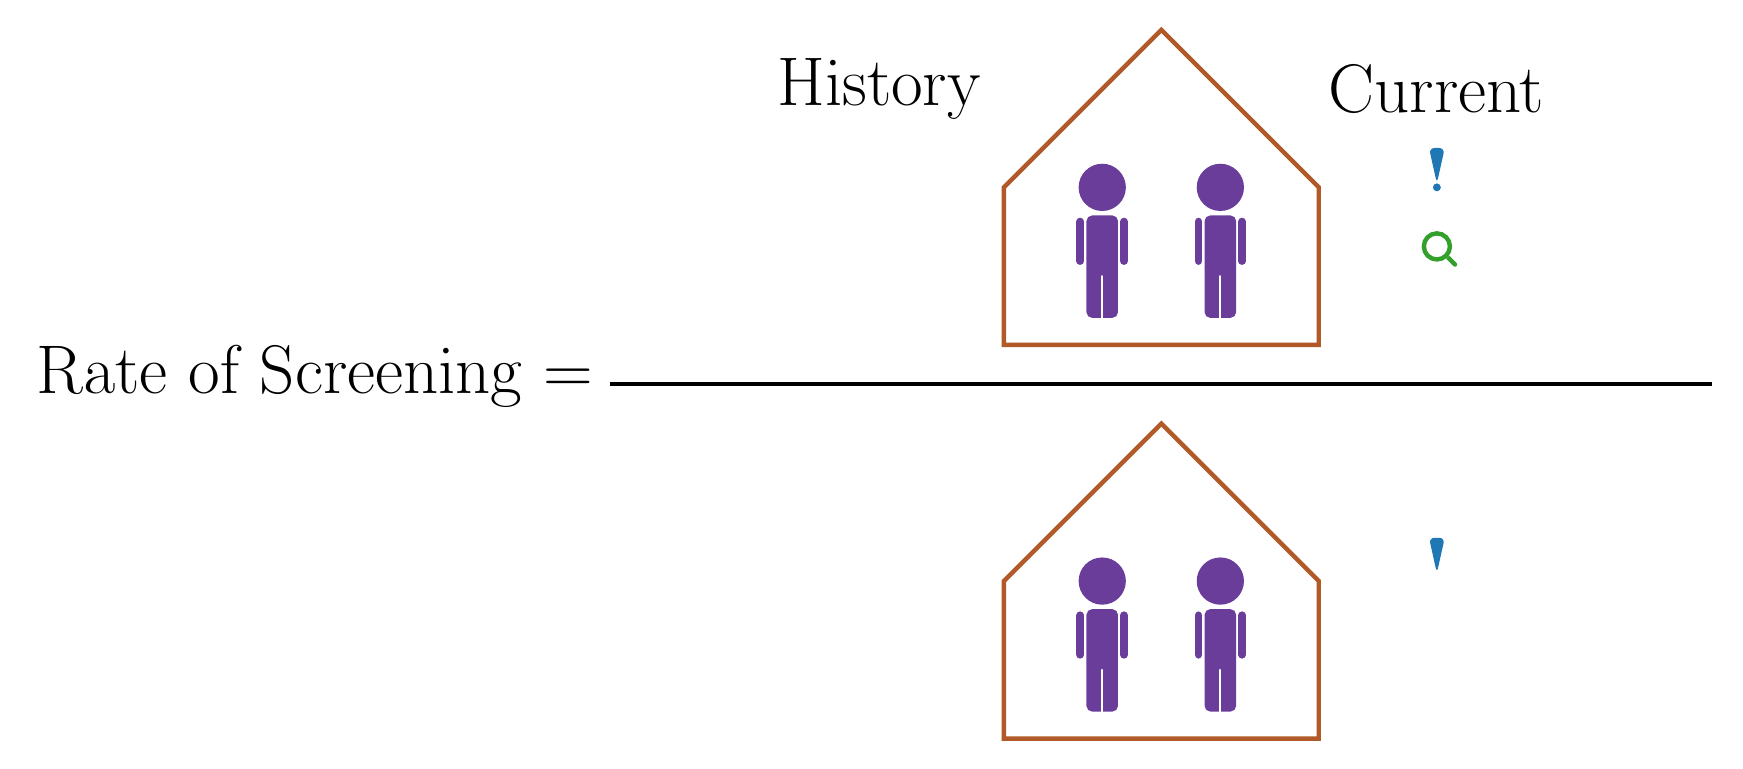
\begin{tikzpicture}

\tikzstyle{lens} = [draw=nice_green, circle, minimum size=2mm, ultra thick]
\tikzstyle{dot} = [draw, circle, minimum size=1mm, inner sep=0pt]

\definecolor{nice_brown}{HTML}{B15928}
\definecolor{nice_purple}{HTML}{6A3D9A}
\definecolor{nice_blue}{HTML}{1F78B4}
\definecolor{nice_green}{HTML}{33A02C}
\definecolor{nice_orange}{HTML}{FF7F00}





%house and people numerator
\draw[ultra thick,draw=nice_brown] (0,2) -- (0,0) -- (4,0) -- (4,2) -- (2,4) -- (0,2) -- (0,0);

%%people
\draw[thick, fill=nice_purple, draw=none] (1.25,2) circle (3mm);
\draw[thick, fill=nice_purple, draw=none] (2.75,2) circle (3mm);
\coordinate (head1center) at (1.25,2);
\coordinate (head2center) at (2.75,2);
\node[rounded corners=2pt,minimum height=1.3cm,minimum width=0.4cm,fill=nice_purple,below = 3.5mm of head1center] (body1) {};
\node[rounded corners=2pt,minimum height=1.3cm,minimum width=0.4cm,fill=nice_purple,below = 3.5mm of head2center] (body2) {};
\draw[draw=nice_purple, line width=1mm,round cap-round cap] ([shift={(2pt,-1pt)}]body1.north east) --++(-90:6mm);
\draw[draw=nice_purple, line width=1mm,round cap-round cap] ([shift={(-2pt,-1pt)}]body1.north west)--++(-90:6mm);
\draw[thick,white,-round cap] (body1.south) --++(90:5.5mm);
\draw[draw=nice_purple, line width=1mm,round cap-round cap] ([shift={(2pt,-1pt)}]body2.north east) --++(-90:6mm);
\draw[draw=nice_purple, line width=1mm,round cap-round cap] ([shift={(-2pt,-1pt)}]body2.north west)--++(-90:6mm);
\draw[thick,white,-round cap] (body2.south) --++(90:5.5mm);

%fraction

\draw[ultra thick,] (-5,-.5) -- (9,-.5);

%house and people denominator
\draw[ultra thick,draw=nice_brown] (0,-3) -- (0,-5) -- (4,-5) -- (4,-3) -- (2,-1) -- (0,-3) -- (0,-5);

\draw[thick,  fill=nice_purple, draw=none] (1.25,-3) circle (3mm);
\draw[thick,  fill=nice_purple, draw=none] (2.75,-3) circle (3mm);
\coordinate (head1center) at (1.25,-3);
\coordinate (head2center) at (2.75,-3);
\node[rounded corners=2pt,minimum height=1.3cm,minimum width=0.4cm,fill=nice_purple,,below = 3.5mm of head1center] (body1) {};
\node[rounded corners=2pt,minimum height=1.3cm,minimum width=0.4cm,fill=nice_purple,,below = 3.5mm of head2center] (body2) {};
\draw[draw=nice_purple, line width=1mm,fill=nice_purple,round cap-round cap] ([shift={(2pt,-1pt)}]body1.north east) --++(-90:6mm);
\draw[draw=nice_purple, line width=1mm,round cap-round cap] ([shift={(-2pt,-1pt)}]body1.north west)--++(-90:6mm);
\draw[thick,white,-round cap] (body1.south) --++(90:5.5mm);
% 
\draw[draw=nice_purple, line width=1mm,round cap-round cap] ([shift={(2pt,-1pt)}]body2.north east) --++(-90:6mm);
\draw[draw=nice_purple, line width=1mm,round cap-round cap] ([shift={(-2pt,-1pt)}]body2.north west)--++(-90:6mm);
\draw[thick,white,-round cap] (body2.south) --++(90:5.5mm);

%left side of the equation 
\node[] (R_I) at (-8.75,-.4) {\Huge Rate of Screening = };

%right side of the equation 

%magnifying glass
%\node[text=nice_green] at (6.25,1.25)  {\Large = X};
\node[lens] (lens) at (5.5,1.25)  {};
\coordinate (handle) at (5.75,1);
\draw[ultra thick, draw=nice_green, round cap-] (handle) -- (lens);


%magnifying glass bottom
%\node[text=nice_green] at (6.25,-3.7)  {\Large = X};
%\node[lens] (lens) at (5.5,-3.7)  {};
%\coordinate (handle) at (5.75,-3.95);
%\draw[ultra thick, draw=nice_green, round cap-] (handle) -- (lens);


%exclamation
%\node[text=nice_blue] at (6.25,2.25)  {\Large = X};
\coordinate (bar1) at (5.6,2.5);
\coordinate (bar2) at (5.4,2.5);
\coordinate (bar3) at (5.5,2.05);
\draw[fill=nice_blue, draw=none, rounded corners=2pt]  (bar1) --  (bar2) --  (bar3) -- cycle;

\node[dot, draw=none, fill=nice_blue] (dot) at (5.5,2)  {};

%exclamation bottom
%\node[text=nice_blue] at (6.25,-2.7)  {\Large = X};
\coordinate (bar1) at (5.6,-2.45);
\coordinate (bar2) at (5.4,-2.45);
\coordinate (bar3) at (5.5,-2.9);
\draw[fill=nice_blue, draw=none, rounded corners=2pt]  (bar1) --  (bar2) --  (bar3) -- cycle;

%\node[dot, draw=none, fill=nice_blue] (dot) at (5.5,-2.95)  {};


%removal
% \node[text=nice_orange] at (6.25,.2)  {\Large = X};
% \coordinate (removal_symbol_begin) at (5.2,.25);
% \coordinate (removal_symbol_end) at (5.85,.2);
% \path[ultra thick, draw=nice_orange, ->] (removal_symbol_begin) to[bend right] (removal_symbol_end);

%removal bottom
% \node[text=nice_orange] at (6.25,-4.75)  {\Large = X};
% \coordinate (removal_symbol_begin) at (5.2,-4.7);
% \coordinate (removal_symbol_end) at (5.85,-4.75);
% \path[ultra thick, draw=nice_orange, ->] (removal_symbol_begin) to[bend right] (removal_symbol_end);
% 

%left side of house

%removal
% \node[text=nice_orange] at (-1,.2)  {\Large = X};
% \coordinate (removal_symbol_begin) at (-2,.25);
% \coordinate (removal_symbol_end) at (-1.35,.2);
% \path[ultra thick, draw=nice_orange, ->] (removal_symbol_begin) to[bend right] (removal_symbol_end);

%removal bottom
% \node[text=nice_orange] at (-1,-4.75)  {\Large = X};
% \coordinate (removal_symbol_begin) at (-2,-4.7);
% \coordinate (removal_symbol_end) at (-1.35,-4.75);
% \path[ultra thick, draw=nice_orange, ->] (removal_symbol_begin) to[bend right] (removal_symbol_end);
% 
% 
%exclamation
% \node[text=nice_blue] at (-1,2.25)  {\Large = X};
% \coordinate (bar1) at (-1.65,2.5);
% \coordinate (bar2) at (-1.85,2.5);
% \coordinate (bar3) at (-1.75,2.05);
% \draw[fill=nice_blue, draw=none, rounded corners=2pt]  (bar1) --  (bar2) --  (bar3) -- cycle;
% \node[dot, draw=none, fill=nice_blue] (dot) at (-1.75,2)  {};


%exclamation bottom
% \node[text=nice_blue] at (-1,-2.7)  {\Large = X};
% \coordinate (bar1) at (-1.65,-2.45);
% \coordinate (bar2) at (-1.85,-2.45);
% \coordinate (bar3) at (-1.75,-2.9);
% \draw[fill=nice_blue, draw=none, rounded corners=2pt]  (bar1) --  (bar2) --  (bar3) -- cycle;
% 
% \node[dot, draw=none, fill=nice_blue] (dot) at (-1.75,-2.95)  {};
% 

%magnifying glass
% \node[text=nice_green] at (-1,1.25)  {\Large = X};
% \node[lens] (lens) at (-1.75,1.25)  {};
% \coordinate (handle) at (-1.5,1);
% \draw[ultra thick, draw=nice_green, round cap-] (handle) -- (lens);
% 

%magnifying glass bottom
% \node[text=nice_green] at (-1,-3.7)  {\Large = X};
% \node[lens] (lens) at (-1.75,-3.7)  {};
% \coordinate (handle) at (-1.5,-3.95);
% \draw[ultra thick, draw=nice_green, round cap-] (handle) -- (lens);


%\draw[draw=nice_orange] (removal_ellipse_center) ellipse (.5 and 1.25);

%words
\node[right] (current_txt) at (-3,3.25) {\Huge {History}};
\node[right] (current_txt) at (4,3.25) {\Huge {Current}};
%\node[text=nice_blue, right] (intake_txt) at (8,2.25) {\Huge Intakes Received};
%\node[text=nice_green, right] (screen_txt) at (8,1.25) {\Huge Screened-In Intakes};
%\node[text=nice_orange, right] (rem_txt) at (8,.25) {\Huge Removals};


\end{tikzpicture}
\end{document}

